\taskpic{На наклонной плоскости с углом $\alpha$ лежит катушка
  (внутренний радиус --- $r$, внешний --- $R$). На катушку намотана
  нить, свободный конец которой с привязанным к нему грузом массы $m$,
  перекинут через невесомый блок на вершине. Масса катушки $M$
  равномерно распределена по окружности радиуса $R$. Трение катушки о
  плоскость отсутствует. При каком значении угла наклона клина центр
  тяжести катушки будет оставаться в покое?}{
  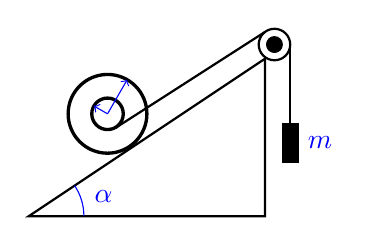
\begin{tikzpicture}
    \draw[thick] (0,0) -- (3,0) -- (3,2) -- cycle;
    \draw[blue] (0.7,0) arc (0:atan(2/3):0.7cm);
    \draw[blue] (0.95,0.25) node {$\alpha$};
    \draw[thick] (3.12,2.18) circle (0.2cm); 
    \filldraw[black] (3.12,2.18) circle (0.1cm);
    \draw[very thick] (1,1.3) circle (0.5cm);
    \draw[very thick] (1,1.3) circle (0.2cm);
    \draw[thick] (1.1,1.12) -- (3,2.34);
    \draw[thick] (3.32,2.18) -- ++(0,-1);
    \filldraw[black] (3.22,1.18) rectangle ++(0.2,-0.5)
    node[midway,right=0.1cm,blue] {$m$};
    \draw[blue,->] (1,1.3) -- ++ (60:0.5cm);
    \draw[blue,->] (1,1.3) -- ++ (150:0.2cm);
\end{tikzpicture}
}
